\documentclass{article}
\usepackage[utf8]{inputenc}
\usepackage{amsthm}
\usepackage{amsmath}
\newtheoremstyle{mystyle}% name
  {\topsep}% Space above
  {\topsep}% Space below
  {\normalfont}% Body font
  {}% Indent amount
  {\bfseries}% Theorem head font
  {}%Punctuation after theorem head
  {.5em}%Space after theorem head
  {}% theorem head spec
\theoremstyle{mystyle}
\newtheorem{prob}{Problem}
\usepackage{graphicx}
\usepackage{wrapfig}
 %preamble
\title{EN.520.214 Project 1}
\author{LJ Gonzales}
\date{March 2023}

\begin{document}
\maketitle
\section{Part 1}
	Note that after having decoded the message, finding the distance between the ship and the located object becomes a trivial task: we can just find the time upon which the echo is heard (number of samples multiplied by $\frac{1}{\text{samples per second}}$) and multiply that by the speed of propagation inside the medium, given at $5000$ feet per second. \\
	We visualize what is in the code in a 3 step process (Figure \ref{3stepfakecode} shows an example with a fabricated message, Figure \ref{3steprealcode} the actual echo to be heard).
	We 1) plot the message to be decoded, 2) it being convolved with the original ping signal, and 3) our best attempt at a reconstructed message, given the output of the matched filter.
\begin{figure}[h]
	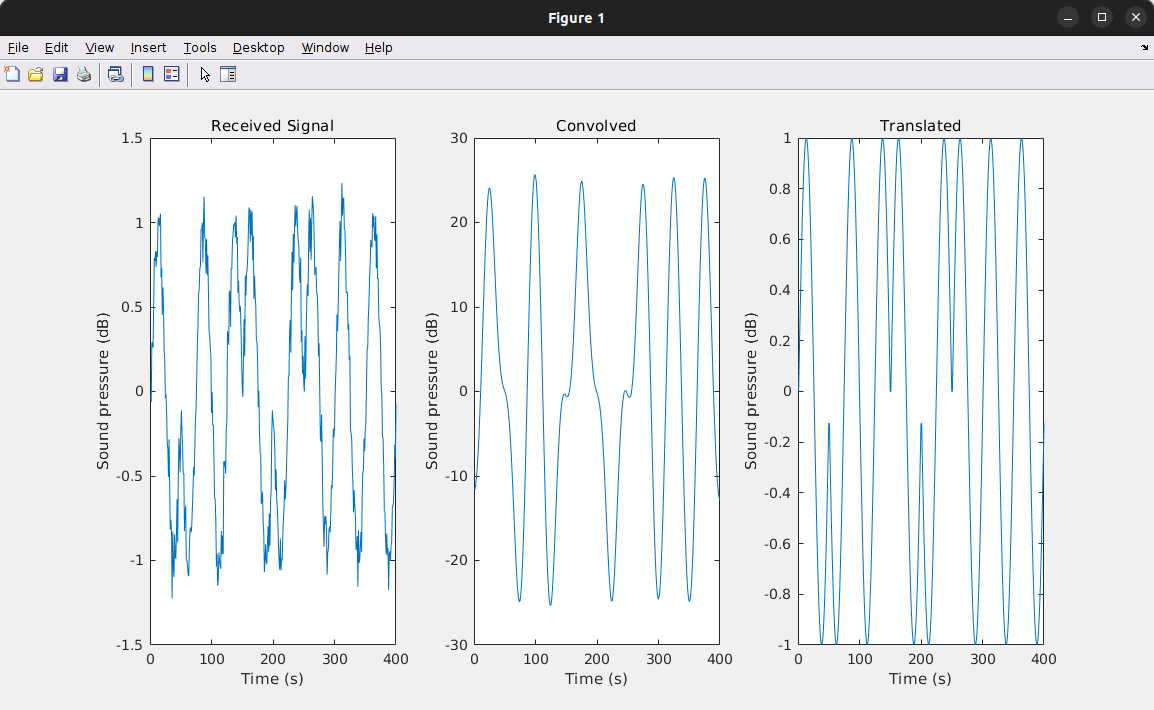
\includegraphics[width =\textwidth]{3stepfakecode.png}
	\label{3stepfakecode}
	\caption{a) Received, b) Convolved, and c) Interpreted from convolved with dummy message}
\end{figure}
\begin{figure}[h]
	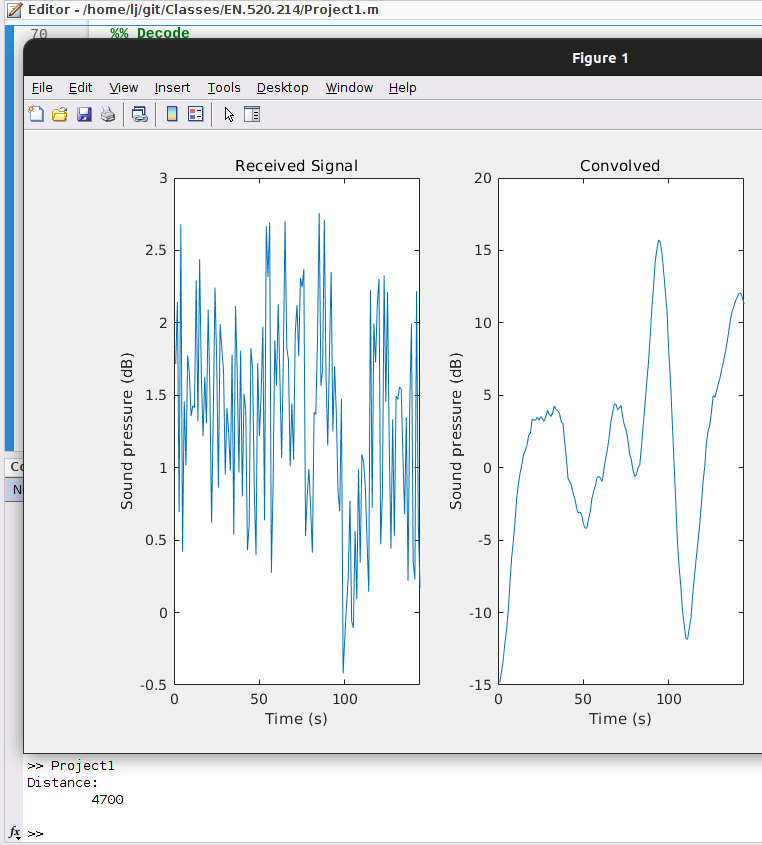
\includegraphics[width =\textwidth]{3steprealcode.png}
	\label{3steprealcode}
	\caption{Same as previous, with SonarEcho. Note how a false 0 is interpreted.}
\end{figure}

	Our test with the fake, non-noisy code best illustrates that when the bipolar signal is in its low state, the convolution reaches a peak low, and a peak high in its high state. This is consistent with our understanding of what the convolution operation does in terms of overlapping sums.
	Note that in order to convolve the message with Matlab's \emph{convolve}, we needed to provide the ping flipped over the time axis and shifted by one period. However, because the ping begins at 0 in the provided file, the \emph{fliplr} function does both of these simultaneously.
	To evaluate the contents of the message, we need to divide it in equal intervals of length $\text{length(SonarPing)}$.
	The problem is that we do not know \emph{a priori} how to do this, because the time between sending and receiving is not necessarily an integer multiple of the length of the code, depending on how far the object is that reflected it.
	We know, however, that the recording \emph{does} contain the reflected signal (a positive 1) at least once inside it, and that any further communications (if any) are sent without any delay from the first. We can then find the global maximum of the convolved graph and center it accordingly.
	Note that here we are making a non-evident assumption about noise contamination in the signal: We need
	\[
	\int_{t}^{t+T}(p(t))^2dt \geq \int_{t}^{t+T}p(t)n(t)dt \text{  } \forall \text{  } t
	.\] 
That is, the overlap of the ping should not be less than the overlap of the noise and ping at any given time.
We can get around proving this requirement by making the further assumption that the noise frequency is much higher than the ping frequency:
we can then use the fact that our signal is symmetric around 0 in amplitude, making the right hand side of the above equation approximately 0 for any choice of t 
(the overlap on the positive half of the ping averages out to be equal and opposite to the overlap on the negative side).
In practice, if we don't have a positive-negative symmetric signal, as in the following parts, we can also ignore this requirement by making the ping amplitude much larger than the worst-case noise amplitude.
\end{document}
